\documentclass{article}
\usepackage{fancyhdr}
\usepackage{amsmath,amssymb}
\usepackage{geometry}
\usepackage{datetime}
\usepackage{enumerate}
\usepackage{graphicx}
\usepackage{hyperref}

\hypersetup{
	colorlinks=true,
	urlcolor=magenta
}

%Insert page formatting here
%\hoffset = -.5in
\voffset = -0.375in
%\textwidth = 6in
\textheight = 8in
\headheight = 24pt

\pagestyle{fancy}

\rhead{Peter Olson\\Student ID: $441666$}
\lhead{Math 3200\\Homework 3}
\chead{\today}
\cfoot{}

%\addtolength{\headwidth}{\marginparsep}
%\addtolength{\headwidth}{\marginparwidth}

%\renewcommand{\labelitemi}{$\diamond$}
\renewcommand{\implies}{\rightarrow}
\newcommand{\widespace}{\qquad \qquad \;}
\newcommand{\tret}{\\ \hline}
\newcommand{\fh}{\tfrac{1}{2}}
\newcommand{\deriv}[2]{\frac{d #1}{d #2}}
\newcommand{\pderiv}[2]{\frac{\delta #1}{\delta #2}}
\newcommand{\vr}{\vec{r}}
\newcommand{\at}{\text{ at }}

\begin{document}
\section*{Binomial Distribution Written Problem}
\begin{enumerate}[\quad(a)]
	\item Please flip a coin (i.e. a quarter) 10 times and record the number of heads. What did you expect? Is the number of heads in your experiment the same as your expectation?
	
	\begin{tabular}{|c|c|c|c|c|c|c|c|c|c|c|}
		\hline
		0 & 1 & 2 & 3 & 4 & 5 & 6 & 7 & 8 & 9 & Total \\
		\hline
		H & H & T & T & H & H & T & H & H & H & 7 \\
		\hline
	\end{tabular}
	\item Please redo Part a. 20 times and report the number of heads in each experiment. Summarize your experiment using five number summaries and a histogram.
	
	Rather than waste my time flipping a coin, I'm just going to use a dataset compiled by two students at UC Berkley, which is available \href{https://www.stat.berkeley.edu/~aldous/Real-World/coin_tosses.html}{here}, at the link for the complete dataset. Using this dataset, the data below was gathered by partitioning the coin tosses into groups of 10, and recording the number of heads in each partitioned set.\\\\
	\begin{minipage}[c]{0.4\textwidth}
			\begin{tabular}{|c|c|}
				\hline 
				Iteration & Number of Heads \\ 
				\hline 
				1 &  3 \\ 
				\hline 
				2 &  4 \\ 
				\hline 
				3 &  6 \\ 
				\hline 
				4 &  8 \\ 
				\hline 
				5 &  1 \\ 
				\hline 
				6 &  5 \\ 
				\hline 
				7 &  4 \\ 
				\hline 
				8 &  3 \\ 
				\hline 
				9 &  5 \\ 
				\hline 
				10 &  8 \\ 
				\hline 
				11 &  5 \\ 
				\hline 
				12 &  6 \\ 
				\hline 
				13 &  7 \\ 
				\hline 
				14 &  5 \\ 
				\hline 
				15 &  3 \\ 
				\hline 
				16 &  4 \\ 
				\hline 
				17 &  7 \\ 
				\hline 
				18 &  5 \\ 
				\hline 
				19 &  6 \\ 
				\hline 
				20 &  5 \\ 
				\hline 
			\end{tabular} 
	\end{minipage}
	\begin{minipage}{0.4\textwidth}
		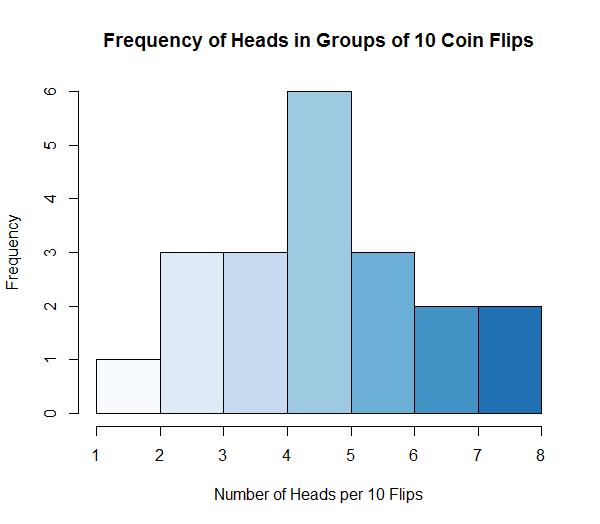
\includegraphics[width=3in]{q6.png}
	\end{minipage}
	\item Do you think you have a fair coin based on your result from parts $a$ and $b$?
	
	I do. Bernoulli trials, with a large enough sample size, will begin to resemble the normal distribution, which is quite evident here.
	\item A physicist claims that a typical quarter actually has a higher chance ($60\%$) that it will hand on "heads", rather than tails, because of the different figures on the two sides of a quarter. Do you agree with him? Why, or why not?
	
	I disagree with him. With a 60\% probability of landing on the heads side, I would expect a greater skew of the data towards the higher numbers, whereas my experiment appears pretty well distributed.
	\item Please use R to simulate this random experiment. First, simulate the number of heads in each 1000 random experiments in which you flip a fair coin 10 times. Then, redo your simulation with the probability of heads being 0.6, mirroring the imaginary physicist's claim in part $d$. Finally, compare your histograms of the two datasets and describe your findings.
	
	Please note that all of the graphs for this question are on the following page, so that they can be presented together.
	
	With the physicist's coin, as expected, the distribution is skewed towards the higher end of the potential range of outcomes, with 10/10 heads being the highest. What I did not initially realize is that this also both makes the tails smaller, and condenses the distribution of the data. Notably, on the graph for solely the fair coin, all 10 potential outcomes occur at least once, whereas with the physicist's coin, there is never fewer than 2 heads in all of the outcomes.
	
	The completely fair coin's distribution looks an awful lot like an approximation of a normal distribution, doesn't it?
	
	Either way, the physicist's imagined coin with a 60\% probability of getting a heads very much does not look like the data that was gathered for part $b)$, and as such, it would tend to discredit his claim that coins favour one side over the other.
	\newpage
	\begin{minipage}{0.46\textwidth}
		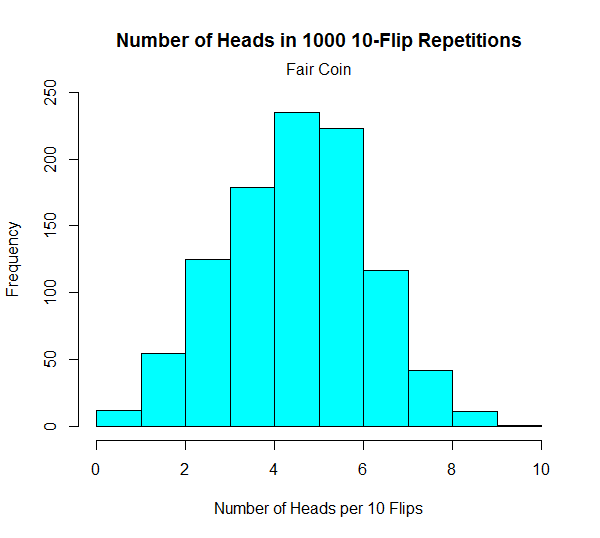
\includegraphics[width=3in]{q61.png}
	\end{minipage}
	\begin{minipage}{0.4\textwidth}
		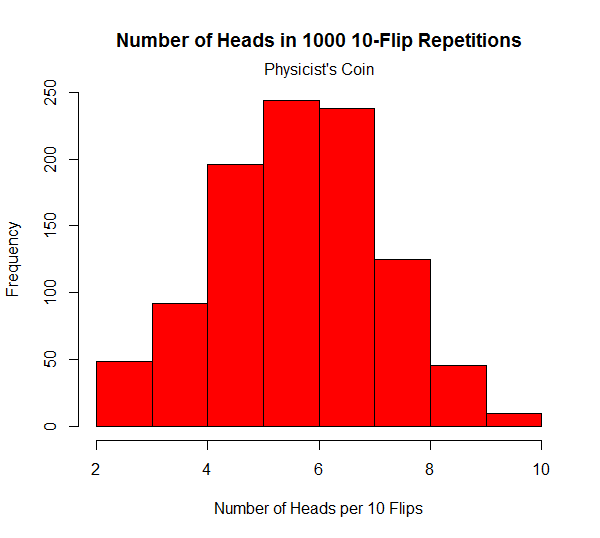
\includegraphics[width=3in]{q62.png}
	\end{minipage}\\
	\begin{minipage}{0.8\textwidth}
		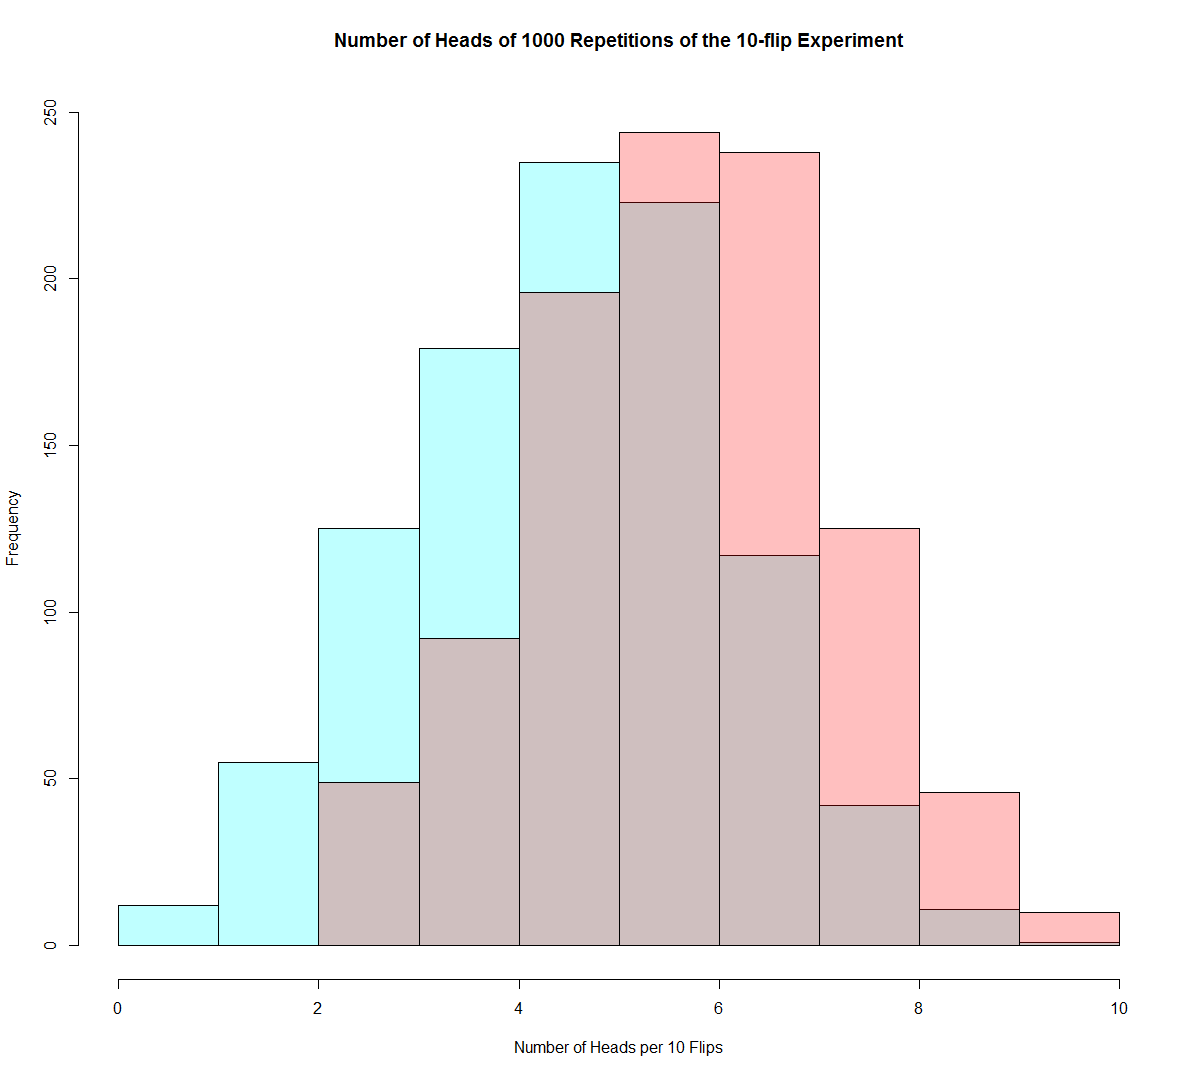
\includegraphics[width=5.5in]{q63.png}
	\end{minipage}
\end{enumerate}
\newpage
\subsection*{R Code}
\begin{verbatim}
# For b)
> heads = c(3,4,6,8,1,5,4,3,5,8,5,6,7,5,3,4,7,5,6,5)
> hist(heads,
+      xlab = "Number of Heads per 10 Flips",
+      main = "Frequency of Heads in Groups of 10 Coin Flips",
+      include.lowest = TRUE,
+      xlim = range(1,8),
+      col = blues9)

# For d)
# n.b. that the plotting here uses the following link for instruction:
# http://stackoverflow.com/questions/3541713/how-to-plot-two-histograms-together-in-r
> fair <- rbinom(n=1000, size = 10, prob = 0.5)
> phys <- rbinom(n=1000, size = 10, prob = 0.6)
# Histogram of both overlaid together
> hist(fair,
+     main = "Number of Heads of 1000 Repetitions of the 10-flip Experiment",
+     xlab = "Number of Heads per 10 Flips",
+     col = rgb(0, 1, 1, 1/4),
+     ylim = c(0,250)
+ )
> hist(phys,
+     col = rgb(1, 0, 0, 1/4),
+     add = T
+ )
# Just fair
> hist(fair,
+     main = "Number of Heads in 1000 10-Flip Repetitions",
+     xlab = "Number of Heads per 10 Flips",
+     col = rgb(0, 1, 1),
+     ylim = c(0,250)
+ )
> mtext("Fair Coin")
# Just physicist's prediction
> hist(phys,
+     main = "Number of Heads in 1000 10-Flip Repetitions",
+     xlab = "Number of Heads per 10 Flips",
+     col = rgb(1, 0, 0),
+     ylim = c(0,250)
+ )
> mtext("Physicist's Coin")
\end{verbatim}

\end{document}